\chapter{Pruebas de software}
\label{chap:chapter3}


El presente capítulo tiene como objetivo validar el correcto funcionamiento del sistema multiagente conversacional desarrollado para interpretar y contextualizar los datos no estructurados del transporte marítimo recogidos en el \textit{Diario de la Marina}. A través de un conjunto de pruebas cuidadosamente diseñadas, se evalúa si el sistema cumple con los requisitos funcionales y no funcionales previamente definidos, así como con los criterios de calidad establecidos por el modelo ISO/IEC 25010~\cite{iso25010-2023}.\\
Para ello, se ejecutan pruebas unitarias, de integración y funcionales sobre los distintos componentes del sistema, prestando especial atención al comportamiento del microservicio de inteligencia artificial encargado del procesamiento conversacional. Asimismo, se emplean métricas como el tiempo de respuesta, la coherencia semántica de las respuestas generadas y la capacidad de recuperación de información relevante.\\
Además, se incluyen pruebas empíricas orientadas a medir la usabilidad desde la perspectiva del usuario final, validando si la interfaz permite una interacción fluida y si el sistema entrega respuestas precisas y contextualizadas ante consultas históricas reales.\\
Los resultados obtenidos en esta fase de verificación y validación permiten no solo comprobar la calidad del producto, sino también identificar oportunidades de mejora y establecer la base para una futura evolución del sistema en contextos reales de explotación académica o investigativa.

\section{Pruebas de software}

Las pruebas tratan de demostrar que un programa hace lo que se intenta que haga, así como descubrir defectos en el programa antes de usarlo. Al probar el software, se ejecuta un programa con datos artificiales. Hay que verificar los resultados de la prueba que se opera para buscar errores, anomalías o información de atributos no funcionales del
programa~\cite{sommerville2011software}. A fin de encontrar los errores del sistema y garantizar un nivel aceptable de calidad y confianza, se realizaron pruebas de software, de caja negra, tanto manuales como estáticas, haciendo uso de las principales técnicas existentes, y aprovechando las pruebas automatizadas, apoyándose en la estrategia de pruebas recomendada por el CMS, Desarrollo dirigido por pruebas (\textit{Test Diver Development}, por sus siglas en inglés TDD).

\section{Estrategia de pruebas}

La elaboración de todo producto de software implica la posibilidad de introducción de errores que provocan fallos en el sistema desarrollado. Por este motivo debe existir una vía para garantizar su calidad y correcto funcionamiento. La realización de pruebas es una actividad que permite verificar el producto bajo ciertas condiciones y en base a los requerimientos identificados para la construcción del mismo, los resultados son observados y registrados para su corrección.

\begin{longtable}{|p{2.5cm}|p{3cm}|p{3cm}|p{6cm}|}
	\caption{Plan de Pruebas} \label{tab:plan-pruebas} \\
	\hline
	\textbf{Prueba} & \textbf{Método} & \textbf{Herramienta} & \textbf{Alcance} \\
	\hline
	\endfirsthead
	
	\hline
	\textbf{Prueba} & \textbf{Método} & \textbf{Herramienta} & \textbf{Alcance} \\
	\hline
	\endhead
	
	Unitaria & Caja blanca con la técnica del camino básico & Módulo TestCase de Django para la realización de pruebas automatizadas & Se automatizarán pruebas para las unidades de código separadas por módulos. \\
	\hline
	Funcional & Caja negra con particiones equivalentes & SeleniumIDE & Se probará el funcionamiento del 100\% de los requisitos. \\
	\hline
	Rendimiento & Pruebas de carga y estrés & Apache JMeter & Se aplicará sobre un entorno de pruebas con prestaciones similares a las de despliegue establecidas en los requisitos no funcionales. Se probará la aplicación con 20 usuarios concurrentes buscando tiempos de respuesta menores a 5 segundos. \\
	\hline
	Seguridad &  & Acunetix Web Vulnerability Scanner 9.5 & Se aplicará para detectar vulnerabilidades:
	\begin{itemize}[left=0pt]
		\item Inyección SQL
		\item Programación Cross-Site (XSS)
		\item Ataques de fuerza bruta a las credenciales
		\item Redirecciones y reenvíos no validados
	\end{itemize} \\
	\hline
	Aceptación & Pruebas de alfa y beta &  & Se aplicará la prueba a los encargados del evento como miembros del comité científico y del comité organizador. \\
	\hline
\end{longtable}

\section{Pruebas unitarias}

Se aplican a un componente del software. Podemos considerar como componente, a una función, una clase,
una librería, etc. Estas pruebas las ejecuta el desarrollador, cada vez que va probando fragmentos de código
o scripts para ver si todo funciona como se desea. El objetivo de las pruebas unitarias es aislar cada parte
del programa y mostrar que las partes individuales son correctas. Proporcionan un contrato escrito, que el
fragmento de código debe satisfacer. El método utilizado para realizar este tipo de prueba se denomina caja
blanca~\cite{sommerville2011software}.

\textbf{Método de caja blanca}

Las pruebas de caja blanca intentan garantizar que:

\begin{itemize}
	\item Se ejecutan al menos una vez todos los caminos independientes de cada módulo.
	\item Se utilizan las decisiones en su parte verdadera y en su parte falsa.
	\item Se ejecuten todos los bucles en sus límites.
	\item Se utilizan todas las estructuras de datos internas.
\end{itemize}

Para la realización de las pruebas unitarias, se le aplicó la técnica de prueba del camino básico a las unidades
código que responden a funcionalidades críticas del software, lo cual permitió generar el grafo de flujo,
calcular la Complejidad Ciclomática (CC) para determinar los caminos linealmente independientes y el
número mínimo de escenarios de los casos de prueba para forzar la ejecución de cada camino del conjunto
básico.
Luego en apoyo a las pruebas se usó el módulo TestCase que ofrece el framework, django, para la automatización de las pruebas unitarias. Con él se probó cada módulo desarrollado, y gracias a la aplicación de la
técnica de camino básico, en aquellas funcionalidades críticas, se pudieron automatizar pruebas para cada
uno de los escenarios o caminos posibles, garantizando probar todo el código en cuestión.

Entre los elementos de código que fueron probadas se encuentra el referente al método \textit{post} de la clase
\textit{Message\_Create\_AV}, que se encarga de crear los mensajes tanto del usario como de las respuestas del sistema al usuario en una conversación asociada.

\begin{table}[h]
	\centering
	\caption{Cálculo de la complejidad ciclomática del método \texttt{post} de la clase \texttt{Message\_Create\_AV}}
	\label{tab:complejidad-ciclomatica}
	\begin{tabular}{|c|}
		\hline
		Método \\
		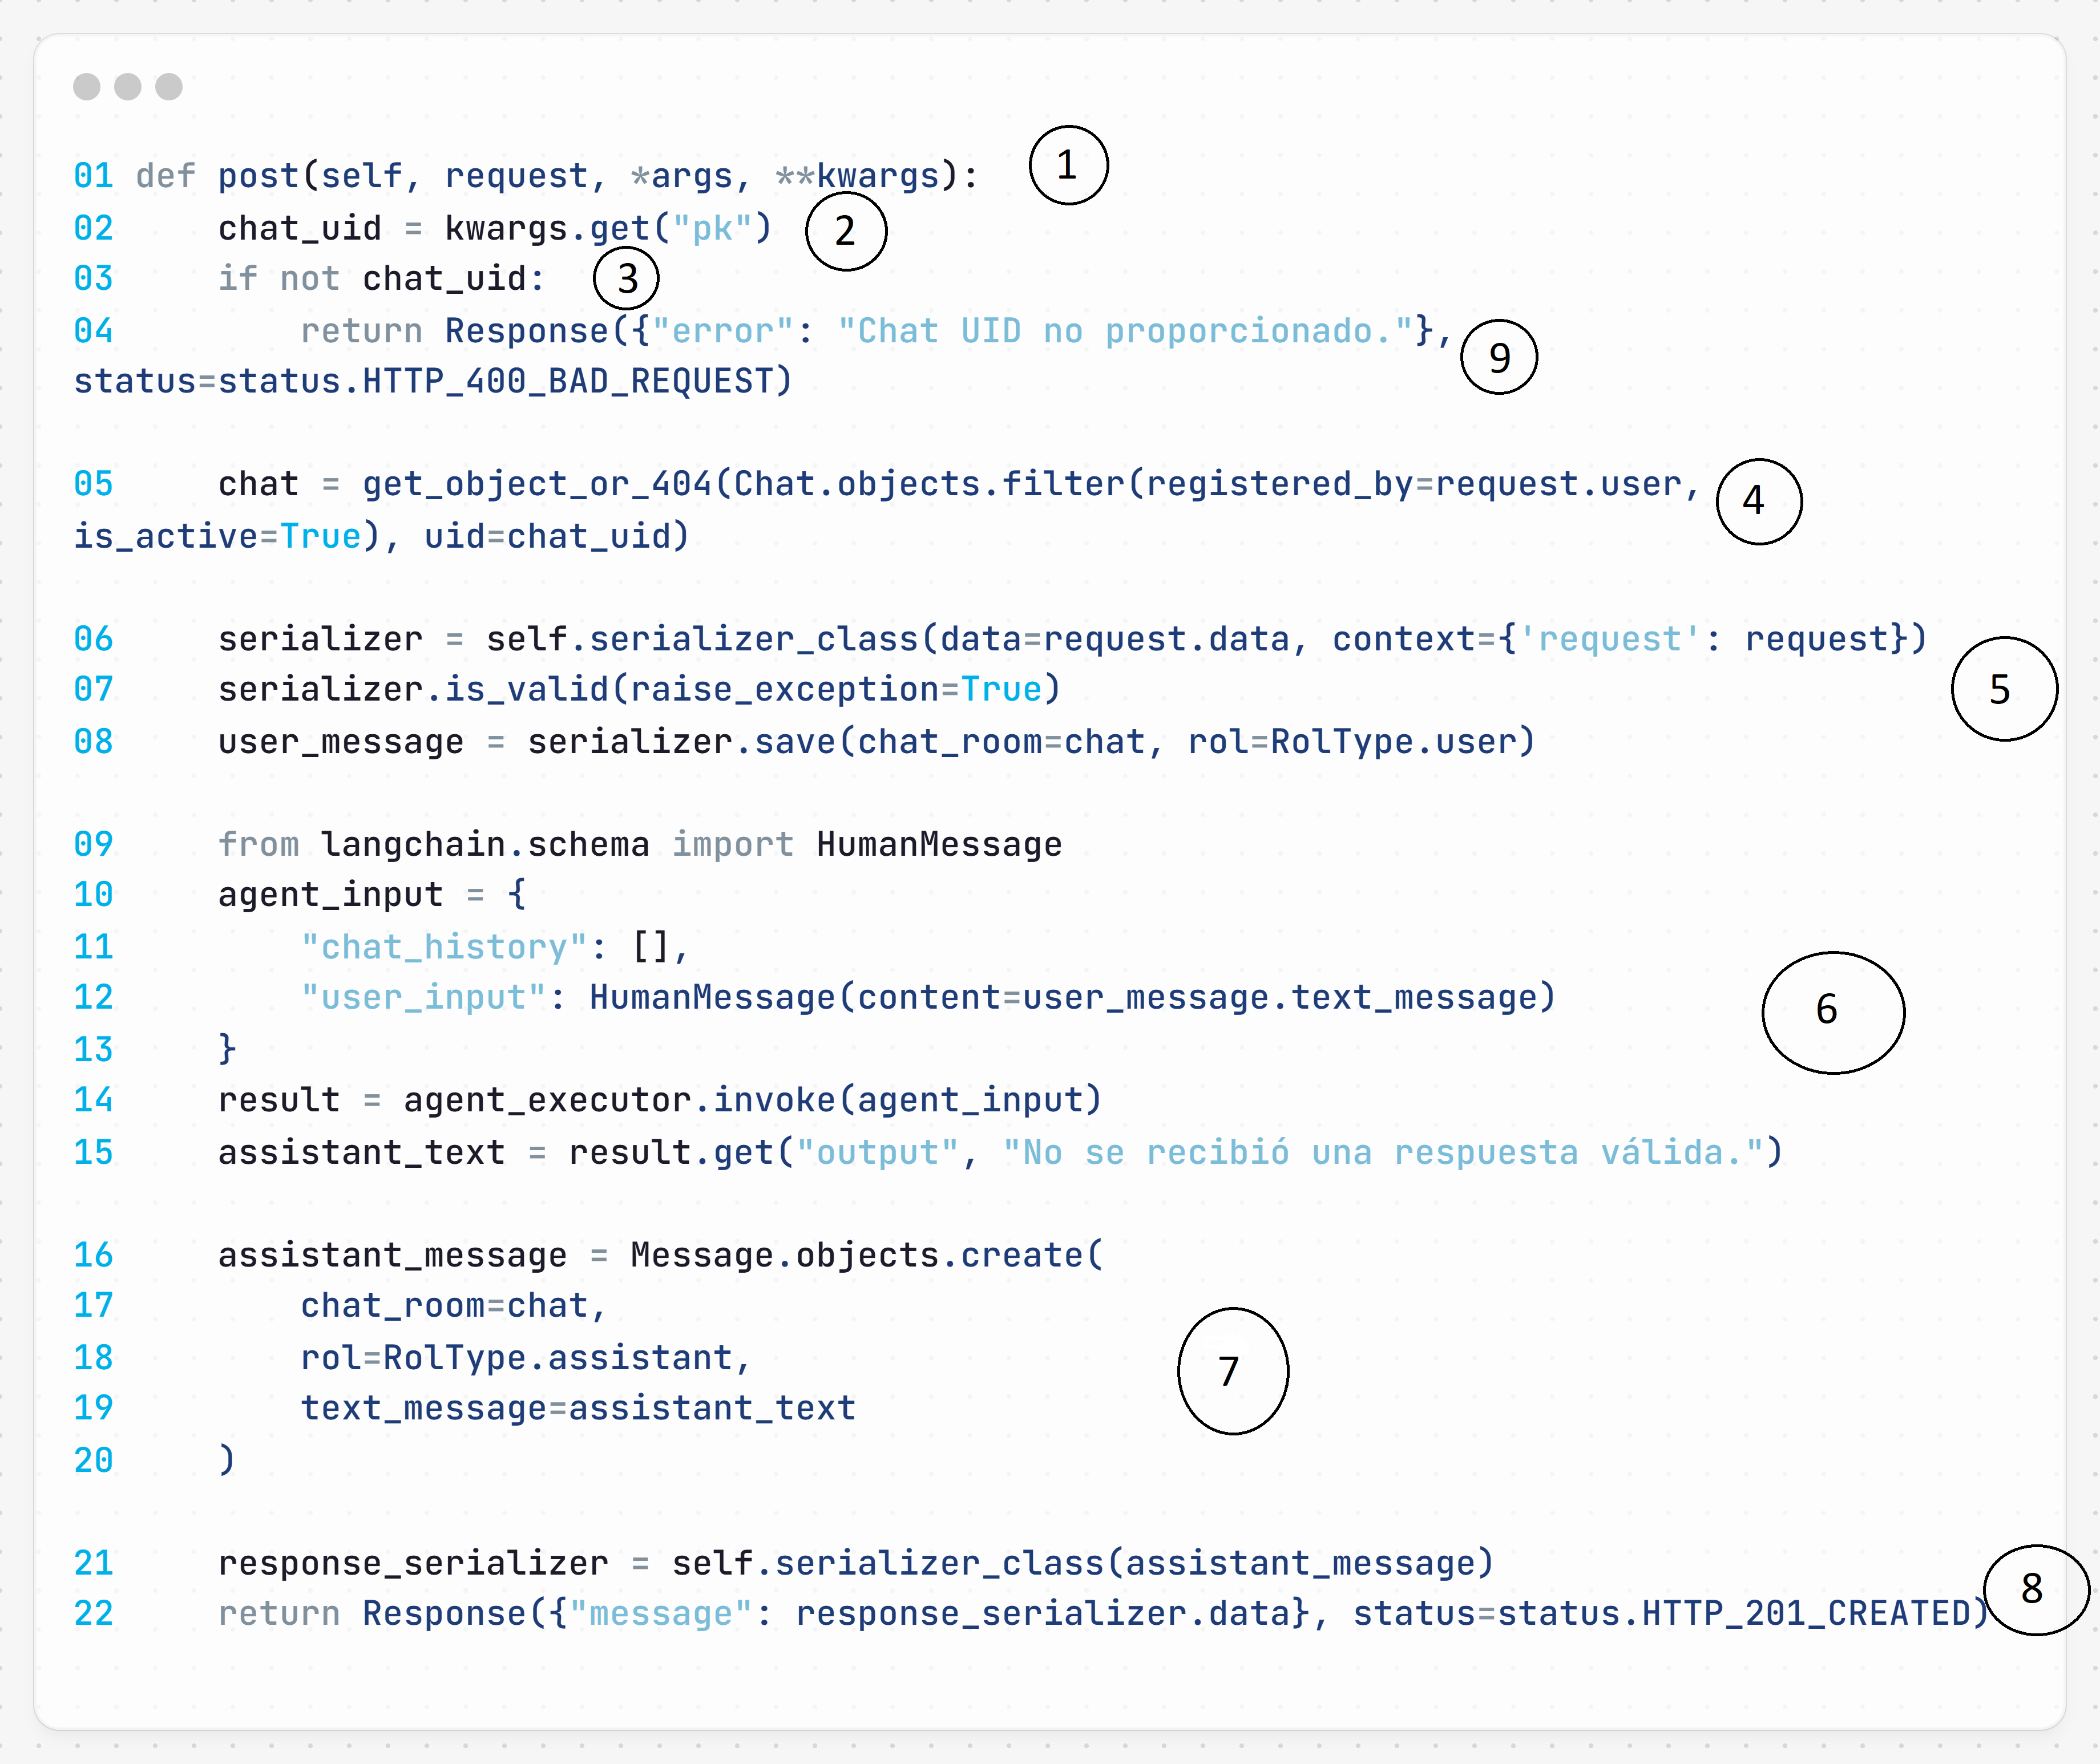
\includegraphics[width=0.4\linewidth]{images/postCreateMessage.png} \\
		\hline
		Grafo \\
		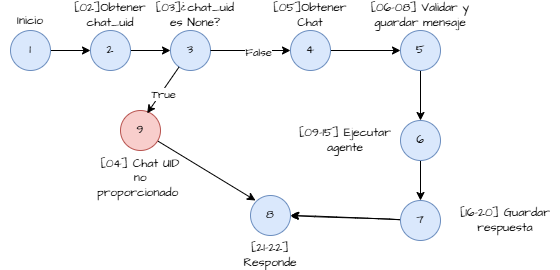
\includegraphics[width=0.4\linewidth]{images/postMessage.png} \\
		\hline
	\end{tabular}
\end{table}

\begin{table}[H]
	\centering
	\caption{Cálculo de la complejidad ciclomática del método \texttt{post} de la clase \texttt{Message\_Create\_AV}}
	\label{tab:complejidad-ciclomatica2}
	\renewcommand{\arraystretch}{1.5}
	\begin{tabular}{|>{\bfseries}m{5cm}|m{4cm}|m{4cm}|}
		\hline
		Complejidad Ciclomática: & \( V(G) = A - N + 2 \) & \( V(G) = P + 1 \) \\
		\hline
		\( V(G) = \# \textit{ de regiones} \) & \( V(G) = 9 - 9 + 2 \) & \( V(G) = 1 + 1 \) \\
		\hline
		\( V(G) = 2 \) & \( V(G) = 2 \) & \( V(G) = 2 \) \\
		\hline
	\end{tabular}
\end{table}

Luego de la determinación de los nodos y flujos de control del código se obtuvo el grafo de flujo y se calculó la complejidad ciclomática del algoritmo.
Como resultado se obtuvo que la CC es igual a 2, lo que significa que existen dos posibles caminos
linealmente independientes y hay que diseñar un mínimo de dos casos de prueba para el algoritmo. La Tabla \ref{tab:caminos-grafo} muestra los caminos existentes.

\begin{table}[h]
	\centering
	\caption{Caminos del grafo de flujo (Fuente: Elaboración propia).}
	\label{tab:caminos-grafo}
	\begin{tabular}{|>{\bfseries}m{5cm}|m{4cm}|m{4cm}|}
		\hline
		\textbf{No.} & \textbf{Camino} \\ \hline
		1            & 1, 2, 3, 9      \\ \hline
		2            & 1, 2, 3, 4, 5, 6, 7, 8   \\ \hline
	\end{tabular}
	\caption{Tabla de caminos}
	\label{tab:caminos}
\end{table}

Los casos de prueba para las pruebas de caja blanca por la técnica de camino básico se ejecutan por cada
camino independiente que se determine en un algoritmo específico. A continuación, se muestra el caso de
prueba para el camino básico independiente 2 del algoritmo.

\begin{longtable}{|p{4cm}|p{11cm}|}
	\caption{Caso de Prueba para el camino básico 2 (Fuente: Elaboración propia).}
	\label{tab:caminos-grafo}\\
	\hline
	\textbf{Proceso} &  \\ \hline
	\textbf{Caso de prueba} & Recibir consulta. Escenario 1.1 \\ \hline
	\textbf{Camino independiente} & 1, 2, 3, 4, 5, 6, 7, 8 \\ \hline
	\textbf{Entradas} &
	\begin{itemize}
		\item \textbf{Consulta}: Lista los barcos que entraron al puerto de la Habana en 1851
	\end{itemize} \\ \hline
	\textbf{Resultados esperados} &
		\begin{itemize}
			\item Lista de barcos que cumplan las condiciones.
			\item En la UI mostrar el mensaje generado por el sistema multiagente.
		\end{itemize} \\ \hline
		
	\textbf{Condiciones de ejecución} &
	\begin{itemize}
		\item El usuario debe estar autenticado.
		\item Debe estar una conversación creada.
	\end{itemize} \\ \hline
\end{longtable}

Con la realización de los casos de prueba diseñados se probó la ejecución de cada sentencia del código al
menos una vez, teniendo en cuenta todas las condiciones lógicas en sus variantes verdaderas y falsas. La
obtención de la CC de valor 2 del método post ejemplificado, permitió determinar que existen 2 caminos
linealmente independientes, suficientes para probar el código al menos una vez.
Los resultados del método de caja blanca fueron satisfactorios. Se automatizaron un total de 25 casos de
prueba con el uso de la biblioteca TestCase, de los cuales a 5 se le aplicó la técnica del camino básico, permitiendo que su automatización garantice probar todos los caminos con un mínimo de escenarios diseñados,
y obteniéndo 0 errores como se aprecia en la Figura \ref{fig:unit_test}.

\begin{figure}[htbp] % h: here, t: top, b: bottom, p: page of floats - ajusta según necesidad
	\centering
	% Asegúrate de que la ruta 'images/arquitectura_web.png' sea correcta
	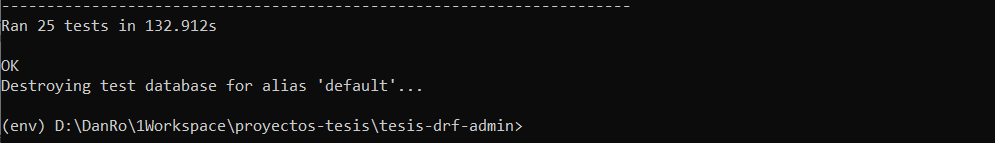
\includegraphics[width=0.9\textwidth]{images/TestCase.PNG} 
	\caption{Resultado de las pruebas unitarias.}
	\label{fig:unit_test}
\end{figure}

\section{Pruebas funcionales}

Este tipo de prueba se realiza sobre el sistema funcionando, comprobando que cumpla con la especificación. Para estas pruebas, se utilizan las especificaciones de casos de prueba. Las pruebas basadas en requerimientos son pruebas de validación más que de defecto: se intenta demostrar que el sistema implementó adecuadamente sus requerimientos~\cite{sommerville2011software}.

\subsection{Método de caja negra}
Las pruebas de caja negra, también llamadas pruebas de comportamiento, se enfocan en los requerimientos funcionales del software. Las técnicas de prueba de caja negra permiten derivar conjuntos de condiciones de entrada que revisarán los requerimientos funcionales para un programa~\cite{pressman2010practitioner}. El método de caja negra presenta varias técnicas de prueba como son: partición de equivalencia, análisis de valores límites y grafos de causaefecto.
En la presente investigación se utilizará específicamente dentro del método de caja negra la técnica de partición de equivalencia generando los casos de pruebas de dicha técnica
sobre las diferentes interfaces que responden a los requisitos funcionales. Para la aplicación de pruebas de regresión sobre los casos de prueba definidos se usará la herramienta Selenium IDE, que permite grabar todas las interacciones de un usuario con el
navegador y posibilita ejecutar de forma automática las mismas, reduciendo el tiempo y los costos de las pruebas funcionales.

\begin{figure}[htbp] % h: here, t: top, b: bottom, p: page of floats - ajusta según necesidad
	\centering
	% Asegúrate de que la ruta 'images/arquitectura_web.png' sea correcta
	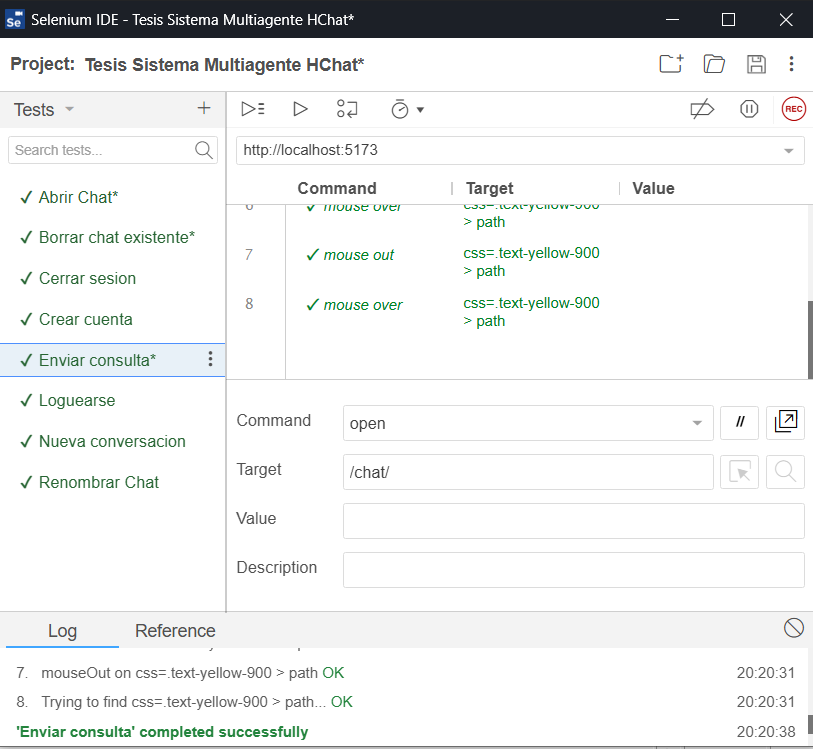
\includegraphics[width=0.9\textwidth]{images/Pruebas_funcionales.PNG} 
	\caption{Representación del resultado la ejecución de una prueba usando Selenium IDE, del requisito Insertar consulta.}
	\label{fig:unit_test}
\end{figure}

A continuación, la Tabla \ref{tab:caso_prueba_enviar_consulta}  muestra el diseño de caso de pruebas del requisito “Insertar consulta” donde se analizarán las variables y condiciones que puedan determinar la respuesta del sistema.


\begin{small} 
	\begin{longtable}{|p{2.2cm}|p{3cm}|p{3.2cm}|p{3.2cm}|p{3.2cm}|}
		\caption{Caso de prueba para la funcionalidad Insertar Consulta (Fuente: Elaboración Propia).} \label{tab:caso_prueba_enviar_consulta} \\
		\hline
		\textbf{Escenario} & \textbf{Descripción} & \textbf{Variables (Mensaje)} & \textbf{Respuesta Esperada} & \textbf{Respuesta} \\
		\hline
		\endfirsthead
		
		\hline
		\textbf{Escenario} & \textbf{Descripción} & \textbf{Variables (Consulta)} & \textbf{Respuesta Esperada} & \textbf{Respuesta} \\
		\hline
		\endhead
		
		\hline
		\endfoot
		
		\hline
		\endlastfoot
		
		EC 1.1. Enviar consulta correctamente & El usuario debe escribir la consulta y dar clic en el botón de enviar & ¿Cuantos barcos entraron al puerto de La Habana en 1851? & 567 & 530 \\
		\hline
		EC 1.2. Enviar consulta incorrecta(con un contexto fuera de la información conocida por el sistema) & El usuario debe escribir la consulta y dar clic en el botón de enviar & ¿Cuánto tiempo duró la 2da guerra mundial? & Lo lamento no tengo esa información disponible & La información solicitada no se encuentra. Por favor reformule la consulta. \\
		\hline
		EC 1.3. Solicitar un consulta cuya respuesta sea una gráfica & El usuario debe escribir la consulta y dar clic en el botón de enviar & Genera una gráfica con el \% de los barcos que entraron a La Habana con arroz en diferentes años. & La respuesta debe ser una gráfica & Responde con una gráfica correspondiente acorde a la consulta \\
		\hline
		\hline
		EC 1.4. Enviar consulta vacía & El usuario debe dar clic en el botón de enviar & - & No se efectúa el envió de consultas vacías & No se envía la consulta vacía \\
		\hline
		
	\end{longtable}
\end{small}

\begin{table}[H]
	\centering
	\begin{tabular}{|c|c|c|p{8.5cm}|}
		\hline
		\textbf{No.} & \textbf{Variable} & \textbf{Valor Nulo} & \textbf{Descripción} \\
		\hline
		1 & Consulta & No & Es un campo de texto que permite al usuario escribir una consulta al sistema \\
		\hline
	\end{tabular}
	\caption{Variables de caso de prueba “Insertar Consulta” (Fuente: Elaboración Propia).}
	\label{tab:variables_insertar_consulta}
\end{table}

Las pruebas de caja negra se aplicaron con el objetivo de evaluar las interfaces de comunicación con el
usuario, las que demostraron coherencia y funcionalidad, así como probar todas aquellas funcionalidades
directamente relacionadas con los requisitos funcionales del sistema. La técnica de partición de equivalencia
es aplicada para evaluar los diferentes escenarios que pueden tener lugar ante la ejecución de una acción.
Como resultado de la aplicación de estas pruebas se ejecutan las posibles variantes que posee una interfaz
de comunicación con el usuario, resolviendo las no conformidades arrojadas y perfeccionando lo obtenido.
Durante la realización de las pruebas se detectaron un conjunto de no conformidades relacionadas con
errores de validación y funcionalidad. Los resultados se muestran en la Figura \ref{fig:grafica_rf}, donde se evidencia la cantidad de casos de prueba ejecutados, los casos de prueba con no conformidades. Se realizaron tres
iteraciones, durante la primera iteración se analizaron 25 casos de prueba, de los cuales 15 resultaron no conformidades. En la segunda y tercera iteración a través de las pruebas de regresión, con el uso del software
Selenium IDE, se verificó que las no conformidades anteriores estuviesen solucionadas, y de estas pruebas
se obtuvieron 6 nuevas no conformidades en la segunda iteración, quedando resuelta en la tercera iteración y
cumpliéndose correctamente los requisitos funcionales.

\begin{figure}[htbp] % h: here, t: top, b: bottom, p: page of floats - ajusta según necesidad
	\centering
	% Asegúrate de que la ruta 'images/arquitectura_web.png' sea correcta
	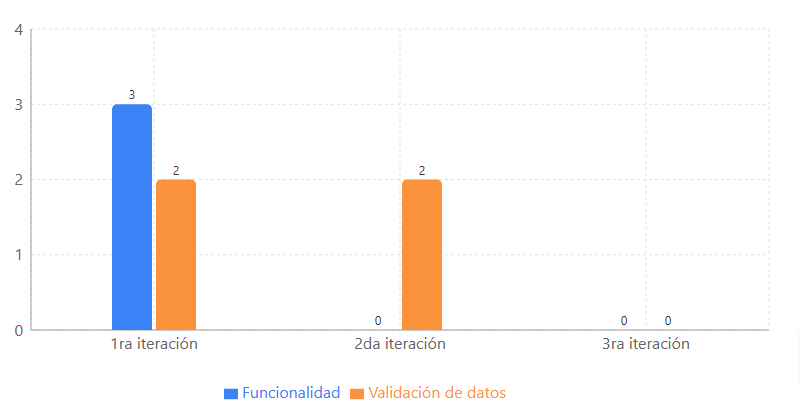
\includegraphics[width=0.9\textwidth]{images/grafica_pruebas_funcionales.PNG} 
	\caption{Representación del resultado de las pruebas funcionales (Fuente: Elaboración Propia).}
	\label{fig:grafica_rf}
\end{figure}

\section{Prueba de seguridad}

Las pruebas de seguridad se diseñan para sondear las vulnerabilidades del entorno del lado del cliente, las
comunicaciones de red que ocurren conforme los datos pasan de cliente a servidor y viceversa, y el entorno
del lado servidor. Cada uno de estos dominios puede atacarse, y es tarea del examinador de seguridad
descubrir las debilidades que puedan explotar quienes tengan intención de hacerlo~\cite{pressman2010practitioner}.\\
Las pruebas de seguridad se aplicaron con ayuda de la herramienta Acunetix Web Vulnerability Scanner 9.5
que establece alertas de tipo: alta, media, baja e informacional, realizándose en dos iteraciones durante el
desarrollo de la propuesta solución.
En una primera iteración se obtuvo un total de 22 alertas de seguridad, de las cuales 4 clasifican de nivel
medio, 1 de nivel bajo y 17 informativas.\\
De las de nivel medio, se destacaron el uso de protocolo no seguro
para el envío de datos, así como los mensajes de error que se muestra en el modo DEBUG de Django para
el desarrollo y se detectaron problemas para la protección de contra ataques de fuerza bruta en el formulario
de autenticación.\\
La de nivel bajo, consistía en vistas del sitio que se podían acceder directamente sin pasar la autenticación
y el sistema de roles establecido. De carácter informativo fueron detectadas posibles cuentas de usuario en ficheros, así como presencia de directorios desprotegidos y la existencia de etiquetas iframe de HTML5.

\begin{figure}[htbp] % h: here, t: top, b: bottom, p: page of floats - ajusta según necesidad
	\centering
	% Asegúrate de que la ruta 'images/arquitectura_web.png' sea correcta
	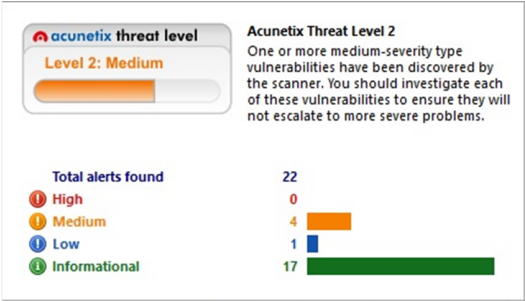
\includegraphics[width=0.9\textwidth]{images/primeraIt.PNG} 
	\caption{ Prueba de seguridad 1ra iteración.}
	\label{fig:grafica_segur}
\end{figure}

Después de aplicar refactorización del código y realizar las validaciones correspondientes, se aplicó la segunda iteración en búsqueda de vulnerabilidades al sistema, arrojando como resultado que todas las que se
habían detectado en la primera iteración, habían sido corregidas.

\begin{figure}[htbp] % h: here, t: top, b: bottom, p: page of floats - ajusta según necesidad
	\centering
	% Asegúrate de que la ruta 'images/arquitectura_web.png' sea correcta
	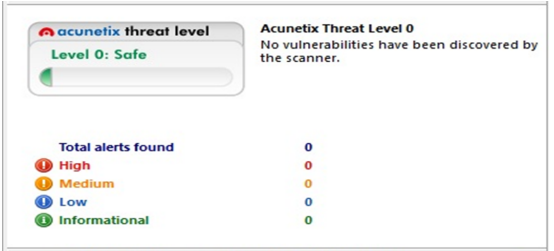
\includegraphics[width=0.9\textwidth]{images/2iter.PNG} 
	\caption{ Prueba de seguridad 2da iteración.}
	\label{fig:grafica_segu2}
\end{figure}

\section{Prueba de rendimiento}

Las pruebas de rendimiento deben diseñarse para garantizar que el sistema procese su carga pretendida. Esto
implica efectuar una serie de pruebas donde se aumenta la carga, hasta que el rendimiento del sistema se
vuelve inaceptable. Las pruebas de rendimiento se preocupan tanto por demostrar que el sistema cumple
con sus requerimientos, como por descubrir problemas y defectos en el sistema~\cite{sommerville2011software}.


\section*{Conclusiones del capítulo}
\addcontentsline{toc}{section}{Conclusiones}